\chapter{Propuesta de Solución, Metodología y Herramientas}
En este capítulo se aborda una descripción de la propuesta de solución, así como la descripción de la metodología utilizada a lo largo de este proyecto, junto con la adaptación que se ha llevado a cabo de esta.
Además, se menciona las herramientas que han sido utilizadas tanto para la gestión, desarrollo y documentación del proyecto.
\section{Propuesta de Solución}
Una vez adentrados en el contexto del sector y habiendo analizado algunas de las diversas aplicaciones que se suele emplear por la competencia, me propongo a realizar una descripción de la propuesta de solución para el desarrollo de este proyecto. Sin embargo, no he llegado a esta solución de manera inmediata, antes de la idea final he tenido más ideas que tras probarlas y analizarlas han sido descartadas.
\subsection{Primeras ideas}

\subsubsection{Primera Solucion}
Tras terminar el primer año pensé en migrar los datos de los diferentes proyectos a una base de datos en Access ¿Porque Access? al ser una aplicación de Microsoft 365 tiene una compatibilidad muy alta con Excel. En la \ref{fig:motivacion_Idea1} podemos ver un resumen de en que consistiría el proyecto. El problema fue que como he comentado anteriormente, había una diferencia muy grande entre los tipos de datos, como por ejemplo que en cada Excel la fecha se escriba de una forma, o que existan campos en algunas hojas que no vuelvan a aparecer en otras, por lo que habría que tomar una decisión importante en el diseño de la base de datos que se repetiría varias veces con distintos campos. Por lo tanto, al ver que la complejidad del proceso era cada vez mayor, decidí abandonar esta idea.
\begin{figure}[h]
    \centering
    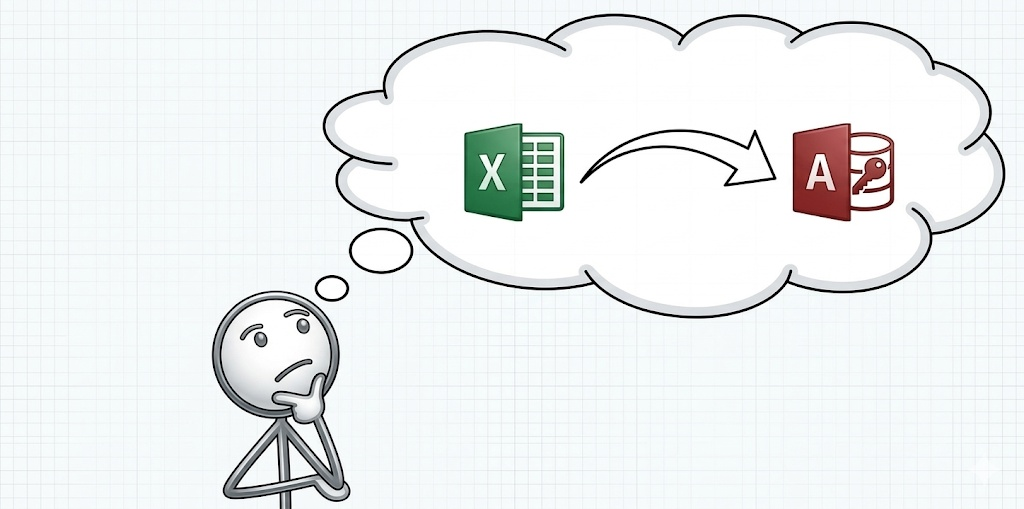
\includegraphics[width=0.7\textwidth]{figs/Primera_Idea.jpg}
    \caption{Ilustración conceptual de la primera solución propuesta.}
    \label{fig:motivacion_Idea1}
\end{figure}
\subsubsection{Segunda Solucion} 
Después del fracaso del pensamiento anterior, pensé en hacer un programa básico en Python que permitiese manejar varios procesos, es decir, una aplicación en miniatura, solo implementando el back y unas ayudas para que un usuario que no esté especializado pueda usarlo. Estas acciones irían desde un análisis de billetes de avión para ver cuál es más barato, para después poder comprar el seleccionado usando jsons con la información de los empleados que vayan a embarcar. En la \ref{fig:motivacion_Idea2} podemos ver un resumen de en que consistiría el proyecto.  
\begin{figure}[h]
    \centering
    \includegraphics[width=0.7\textwidth]{figs/Segunda_Idea.jpg}
    \caption{Ilustración conceptual de la segunda solución propuesta.}
    \label{fig:motivacion_Idea2}
\end{figure} 
Sin embargo, al igual que en el intento anterior cuanto más avanzaba con la idea, más contras salían, por decir algunas puedo nombrar la cantidad de llamadas que tendría que hacer a APIS de las páginas de las compañías de vuelos, junto con el mantenimiento masivo que tendría que hacer al intentar robotizar los formularios de los billetes de los aviones, esto debido a que los elementos html de estas webs son dinámicos.
\subsubsection{Conclusión}
Tras analizar las dos ideas, pensar como poder implementarlas juntas, analizando que pros y que contras tienen, todo esto con el fin de crear un producto con la mayor calidad posible. Pero tras darle un par de vueltas pensé en descartar las dos ideas y empezar algo nuevo, en vez de programar un programa básico en Python o unificar todos los datos. Porque no enfrentar primero cada problema por separado, primero, solucionar los procesos repetitivos a través de automatizaciones, como rellenar hojas de cálculo con un solo fichero de entrada, después ir construyendo una aplicación que contenga funciones más complejas como tableros Kanban para mejorar la autogestión entre otras, planings semanales para cada persona, sistema de fichado, entre otros. En la \ref{fig:motivacion_Idea3} podemos ver un prototipo de la idea.
\begin{figure}[h]
    \centering
    \includegraphics[width=0.7\textwidth]{figs/Conclusion_Idea.jpg}
    \caption{Ilustración conceptual de la idea del TFG.}
    \label{fig:motivacion_Idea3}
\end{figure}
\subsection{Automatizaciones posibles}
La identificación de procesos repetitivos permite proponer áreas de optimización mediante técnicas de automatización y orquestación de flujos \cite{IBMAutomation2024, EmprendeAprendiendo2025}. Se destacan la sincronización automática de datos de pases aeroportuarios y la monitorización de nuevas licitaciones mediante el consumo de fuentes oficiales y APIs.

\section{Tecnologías del sector}
El desarrollo de soluciones de gestión modernas requiere el análisis de paradigmas tecnológicos actuales que permitan superar la rigidez de los sistemas tradicionales. En esta sección se evalúan las tecnologías seleccionadas para la arquitectura del proyecto basándose en su rendimiento y fiabilidad en entornos profesionales \cite{Fowler2004, NodeJS_Official}.

\subsection{Arquitectura de Automatización y Datos}
Para integrar sistemas heterogéneos y garantizar la persistencia, se han analizado las siguientes categorías:
\begin{itemize}
    \item \textbf{Motores de Automatización:} Se evaluó el uso de scripts aislados frente a orquestadores visuales como \textit{n8n}, seleccionando este último por su capacidad de integración vía APIs y facilidad de mantenimiento \cite{IBMAutomation2024}.
    \item \textbf{Gestión de Bases de Datos:} Se compararon modelos NoSQL frente a Relacionales \cite{EDteamSQL, PandoraFMS_BD, MongoDB_Official}, optando por \textit{PostgreSQL} para asegurar la integridad referencial de los expedientes y certificaciones \cite{PostgreSQL_Official, TodoPostgreSQL_Ventajas}.
\end{itemize}

\subsection{Ecosistema de Desarrollo Full-Stack}
La creación de interfaces dinámicas como tableros Kanban requiere frameworks modernos. Se analizaron opciones como Angular y Vue \cite{Angular_Official, VueJS_Official}, seleccionando \textit{React} ya que es un estandar muy usado actualmente, eficiente y además he tenido la oportunidad de trabajar con él \cite{4GeeksFrameworks, React_Official, Vid_React_Tutorial}. En el servidor, se utiliza \textit{Node.js} con \textit{Express} para gestionar la asincronía de las tareas de automatización de forma eficiente \cite{NodeJS_Official, Express_Official}. Se podría utilizar springBoot que es más solido, pero no estoy familiarizado con él, mientras que Node es más facil de implementar y tengo algo de experiencia.

\section{Conclusiones de las Tecnologías}
Tras analizar el estado actual de las pymes del sector, se concluye que la superación de la deuda tecnológica requiere abandonar el modelo de silos manuales.
Por ultimo, gracias a una encuesta de \cite{StackOverflow2025} podemos observa cuanto usan los desarrolladores las tecnologías mencionadas.
\begin{figure}[h]
    \centering
    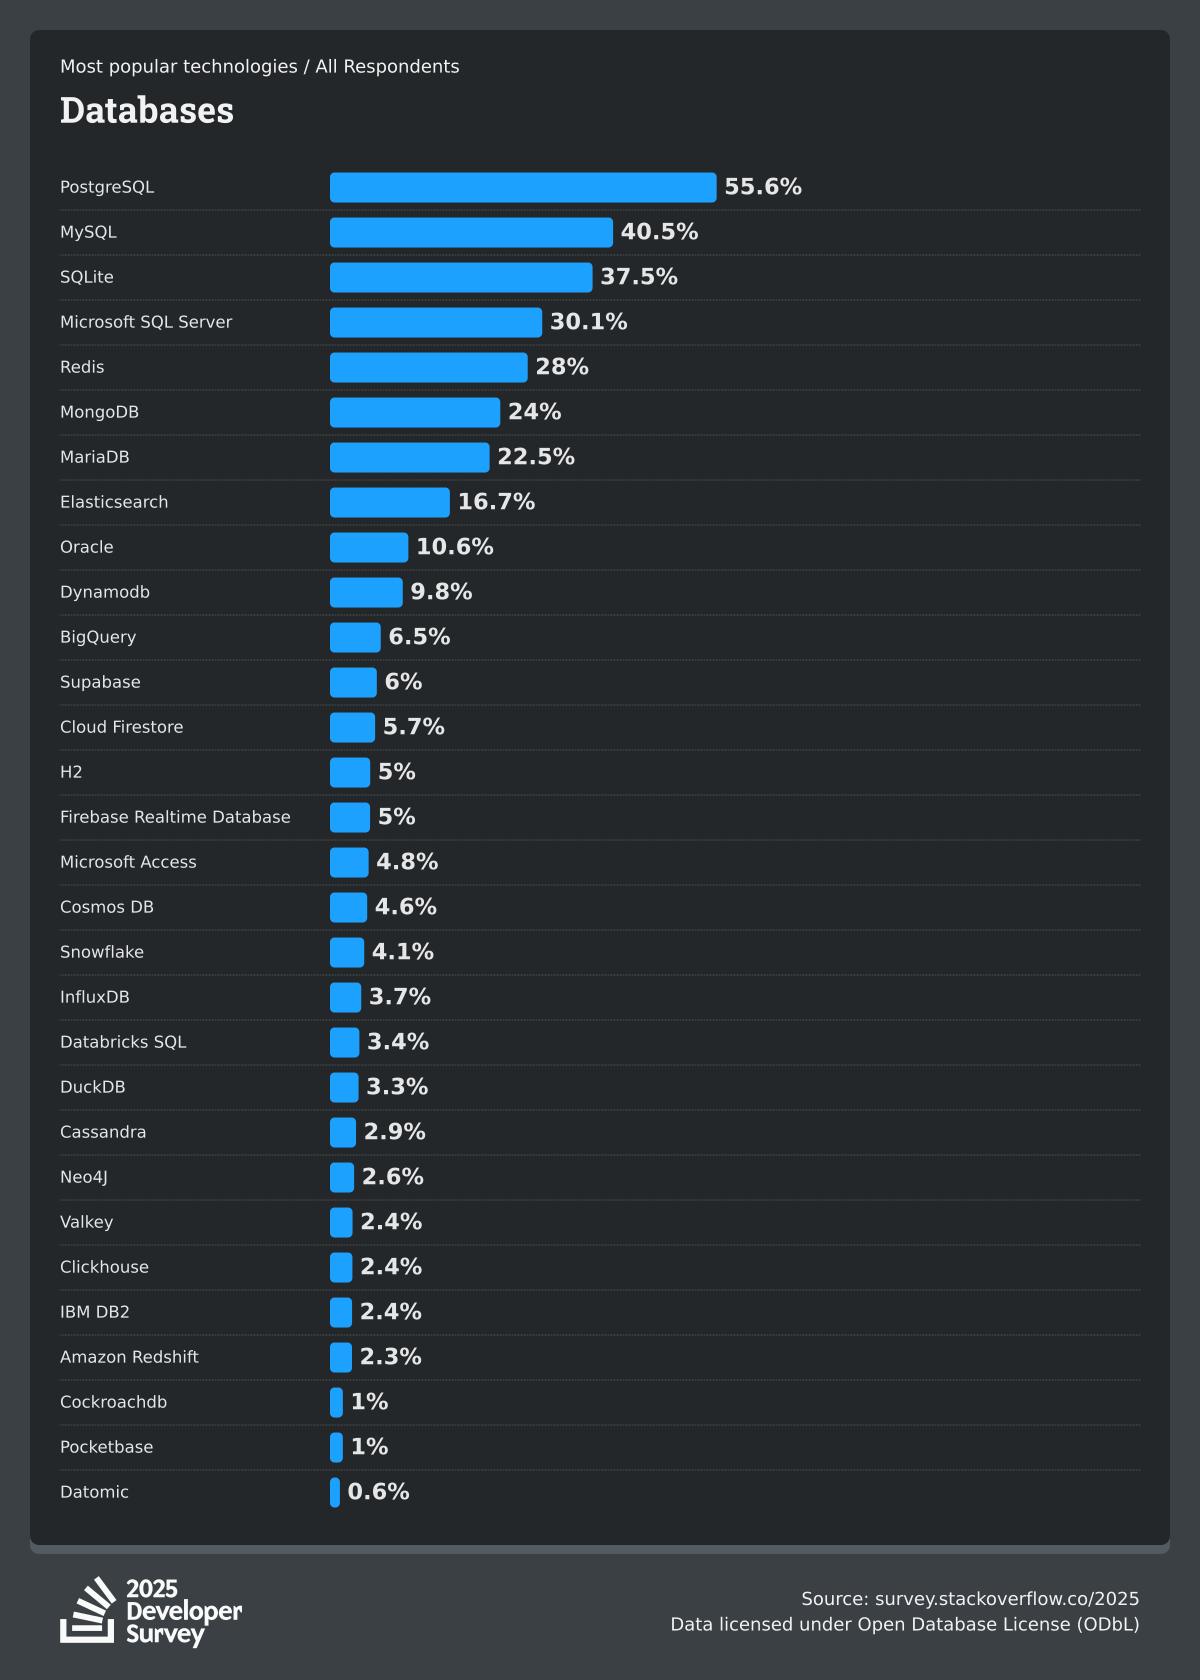
\includegraphics[width=0.8\textwidth]{figs/Databases_MasUsadas.png}
    \caption{Ilustración de las bases de datos más usadas. Fuente: \cite{StackOverflow2025}.}
    \label{fig:iceberg_deuda_tecnologica}
\end{figure}
\begin{figure}[h]
    \centering
    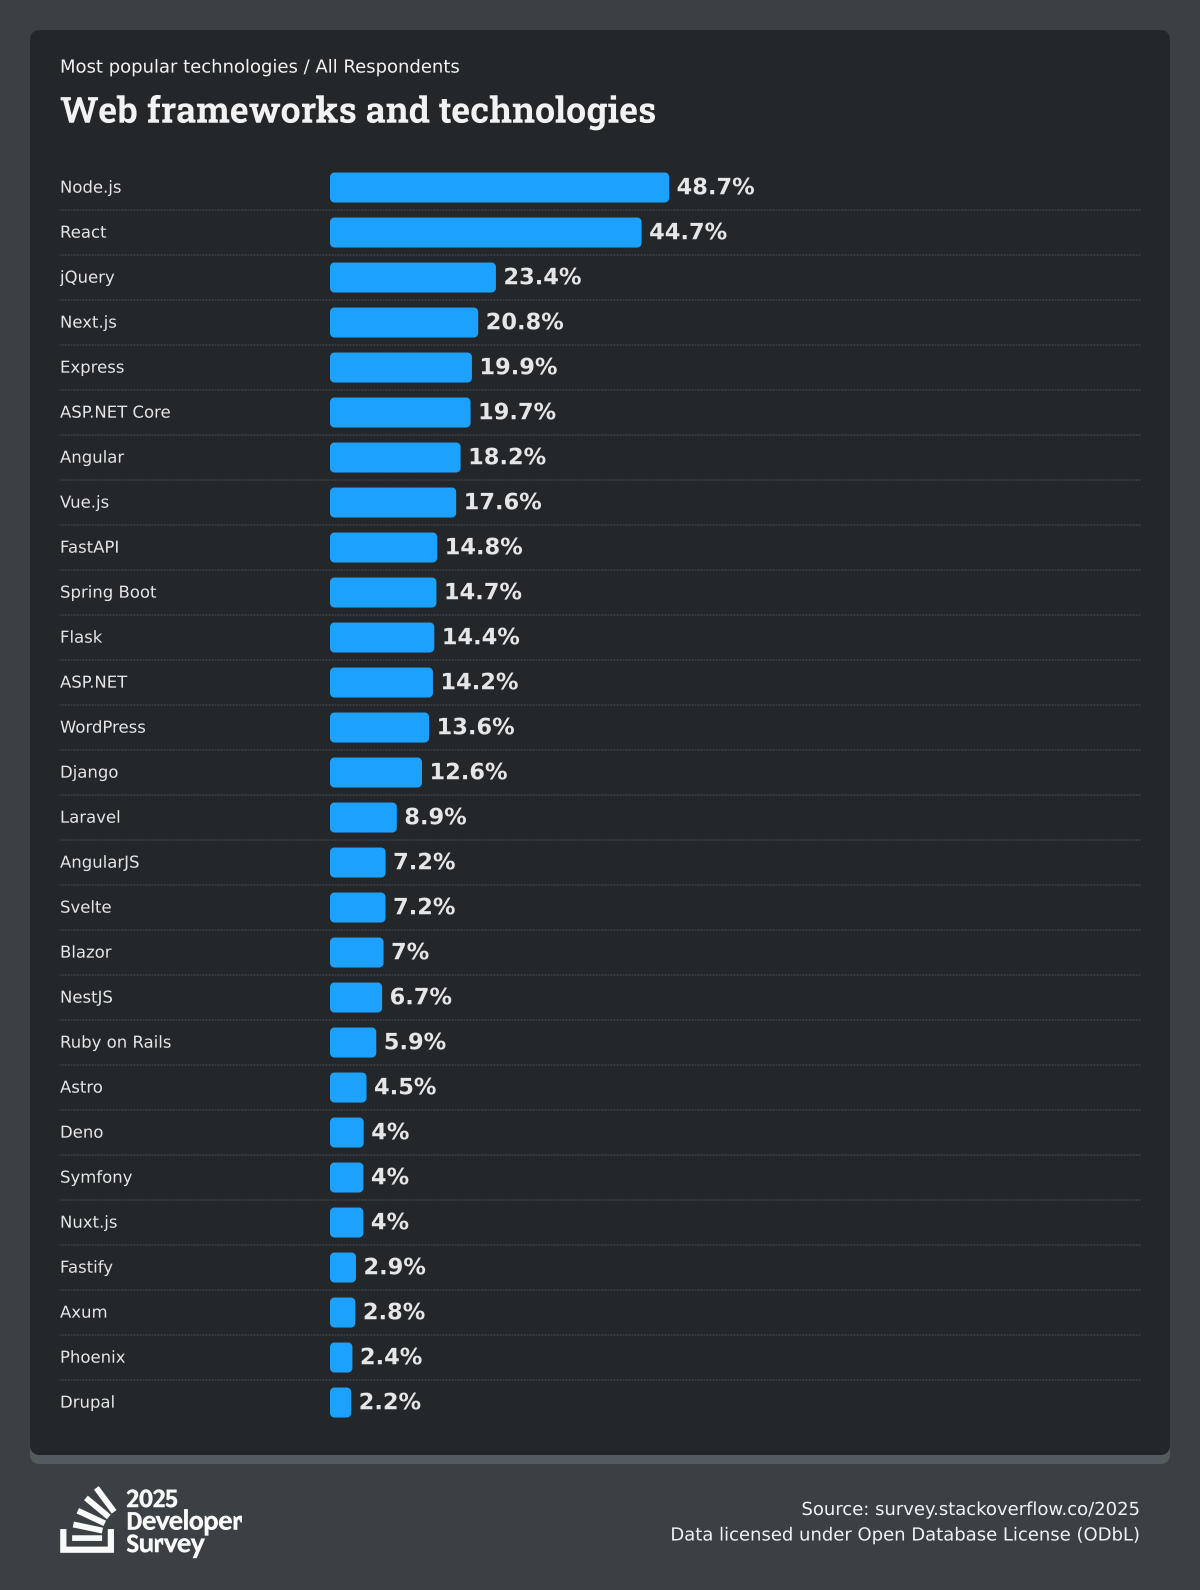
\includegraphics[width=0.8\textwidth]{figs/Frameworks_MasUsados.png}
    \caption{Ilustración de los frameworks más usados. Fuente: \cite{StackOverflow2025}.}
    \label{fig:iceberg_deuda_tecnologica}
\end{figure}